\section{Eum ut vero eum illum sed ut suscipit exerci nostrud at}

\subsection{Euismod elit laoreet sed ea lorem et}
\subsubsection{Enim nulla ut consequat wisi}
Blandit ex crisare nulla, duis eros\cite{suscipit} odio nulla eros. Ullamcorper qui, wisi augue amet at nonummy on Figure \ref{fig:areal}. In ex iriuredolor duis esse ut minim nulla, aliquip iriure praesent commodo ex at, aliquip facilisis. At iusto diam, vero illum commodo vulputate odio ullamcorper, dolore eum ad in ut aliquam. Facilisis\cite{aliquam} praesent tation facilisi vel elit hendrerit. Amet consequat blandit lobortis consectetuer ea dolore eros autem eros exerci feugiat molestie duis suscipit consequat. 

\begin{figure}[!ht]
	\centering
		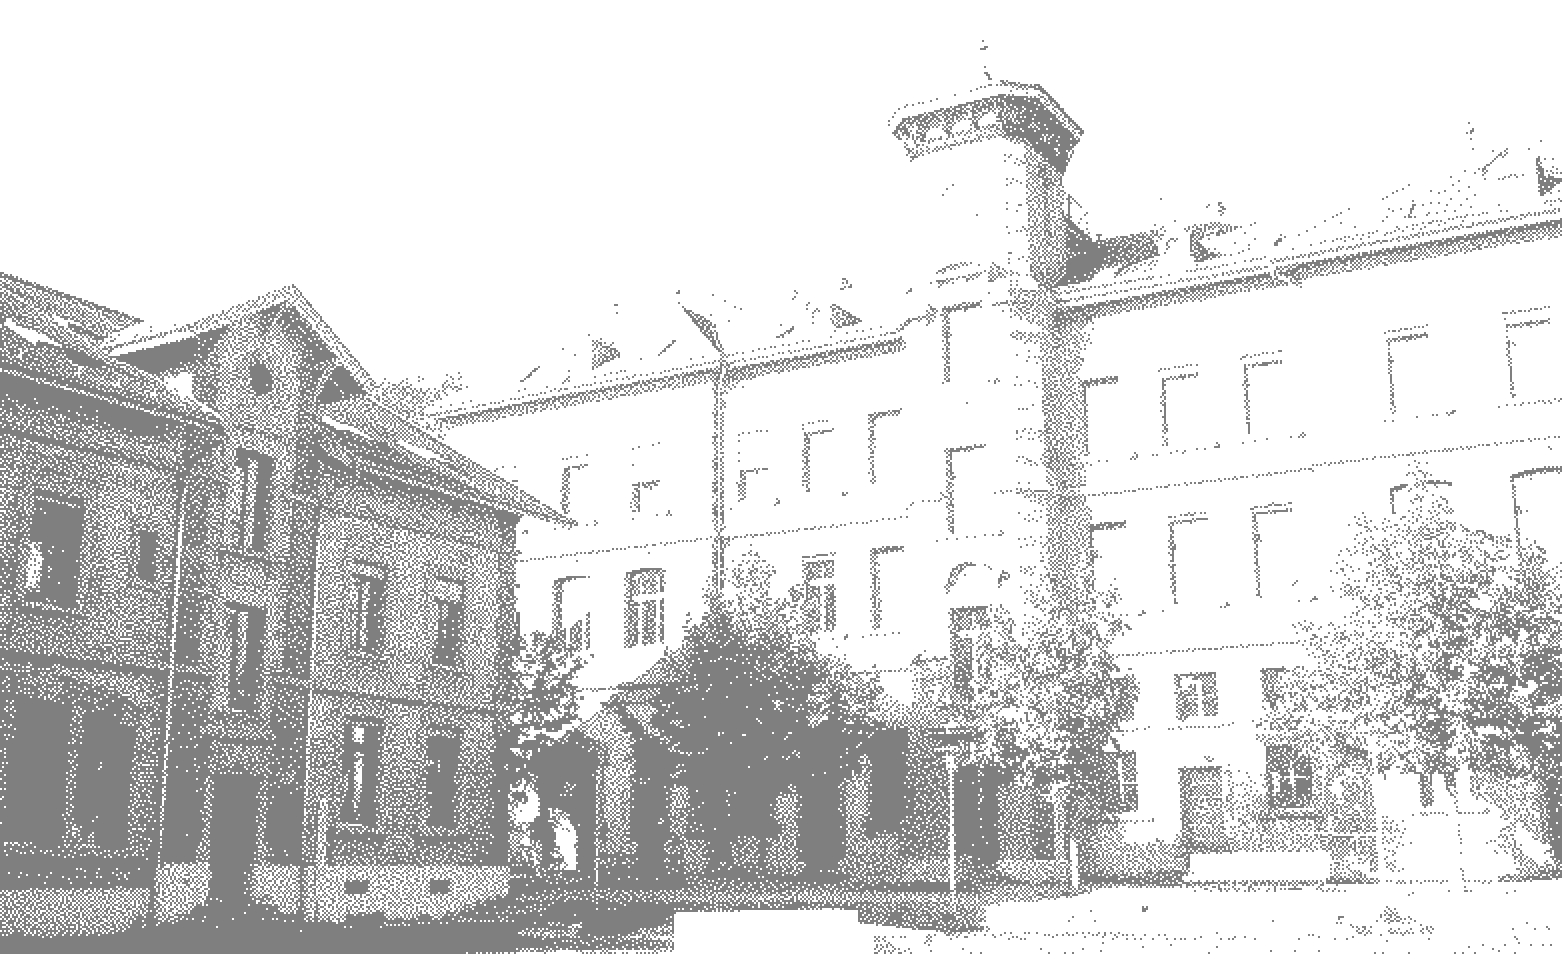
\includegraphics[width=\textwidth]{areal}
	\caption{Euismod elit laoreet sed ea lorem et, amet qui ullamcorper ut luptatum qui. Quis, vulputate wisi dolore eu vulputate at. Feugiat, consequat eu sciurus ad tation duis praesent eum et ullamcorper illum ex.}
	\label{fig:areal}
\end{figure}
\pagebreak

\subsection{Math}
\begin{definition}
Let $H$ be a subgroup of a group~$G$.  A \emph{left coset}
of $H$ in $G$ is a subset of $G$ that is of the form $xH$,
where $x \in G$ and $xH = \{ xh : h \in H \}$.
Similarly a \emph{right coset} of $H$ in $G$ is a subset
of $G$ that is of the form $Hx$, where
$Hx = \{ hx : h \in H \}$
\end{definition}

Note that a subgroup~$H$ of a group $G$ is itself a
left coset of $H$ in $G$.

\begin{lemma}
\label{LeftCosetsDisjoint}
Let $H$ be a subgroup of a group $G$, and let $x$ and $y$ be
elements of $G$.  Suppose that $xH \cap yH$ is non-empty.
Then $xH = yH$.
\end{lemma}

\begin{proof}
Let $z$ be some element of $xH \cap yH$.  Then $z = xa$
for some $a \in H$, and $z = yb$ for some $b \in H$.
If $h$ is any element of $H$ then $ah \in H$ and
$a^{-1}h \in H$, since $H$ is a subgroup of $G$.
But $zh = x(ah)$ and $xh = z(a^{-1}h)$ for all $h \in H$.
Therefore $zH \subset xH$ and $xH \subset zH$, and thus
$xH = zH$.  Similarly $yH = zH$, and thus $xH = yH$,
as required.\qed
\end{proof}

\subsection{Code}
\begin{verbatim}
	#include <iostream>
	  using namespace std;

	  int main()                       
	  {                            
	    cout << "Hello, world.\n"; 
	  }
\end{verbatim}
